\documentclass[twoside, letterpaper, 12pt]{report}
\usepackage{orthodoxservicebook}

\title{The Sunday Reader's Service of the \\ \textsc{Typica} \\ 2020 April 12}
\titlepic{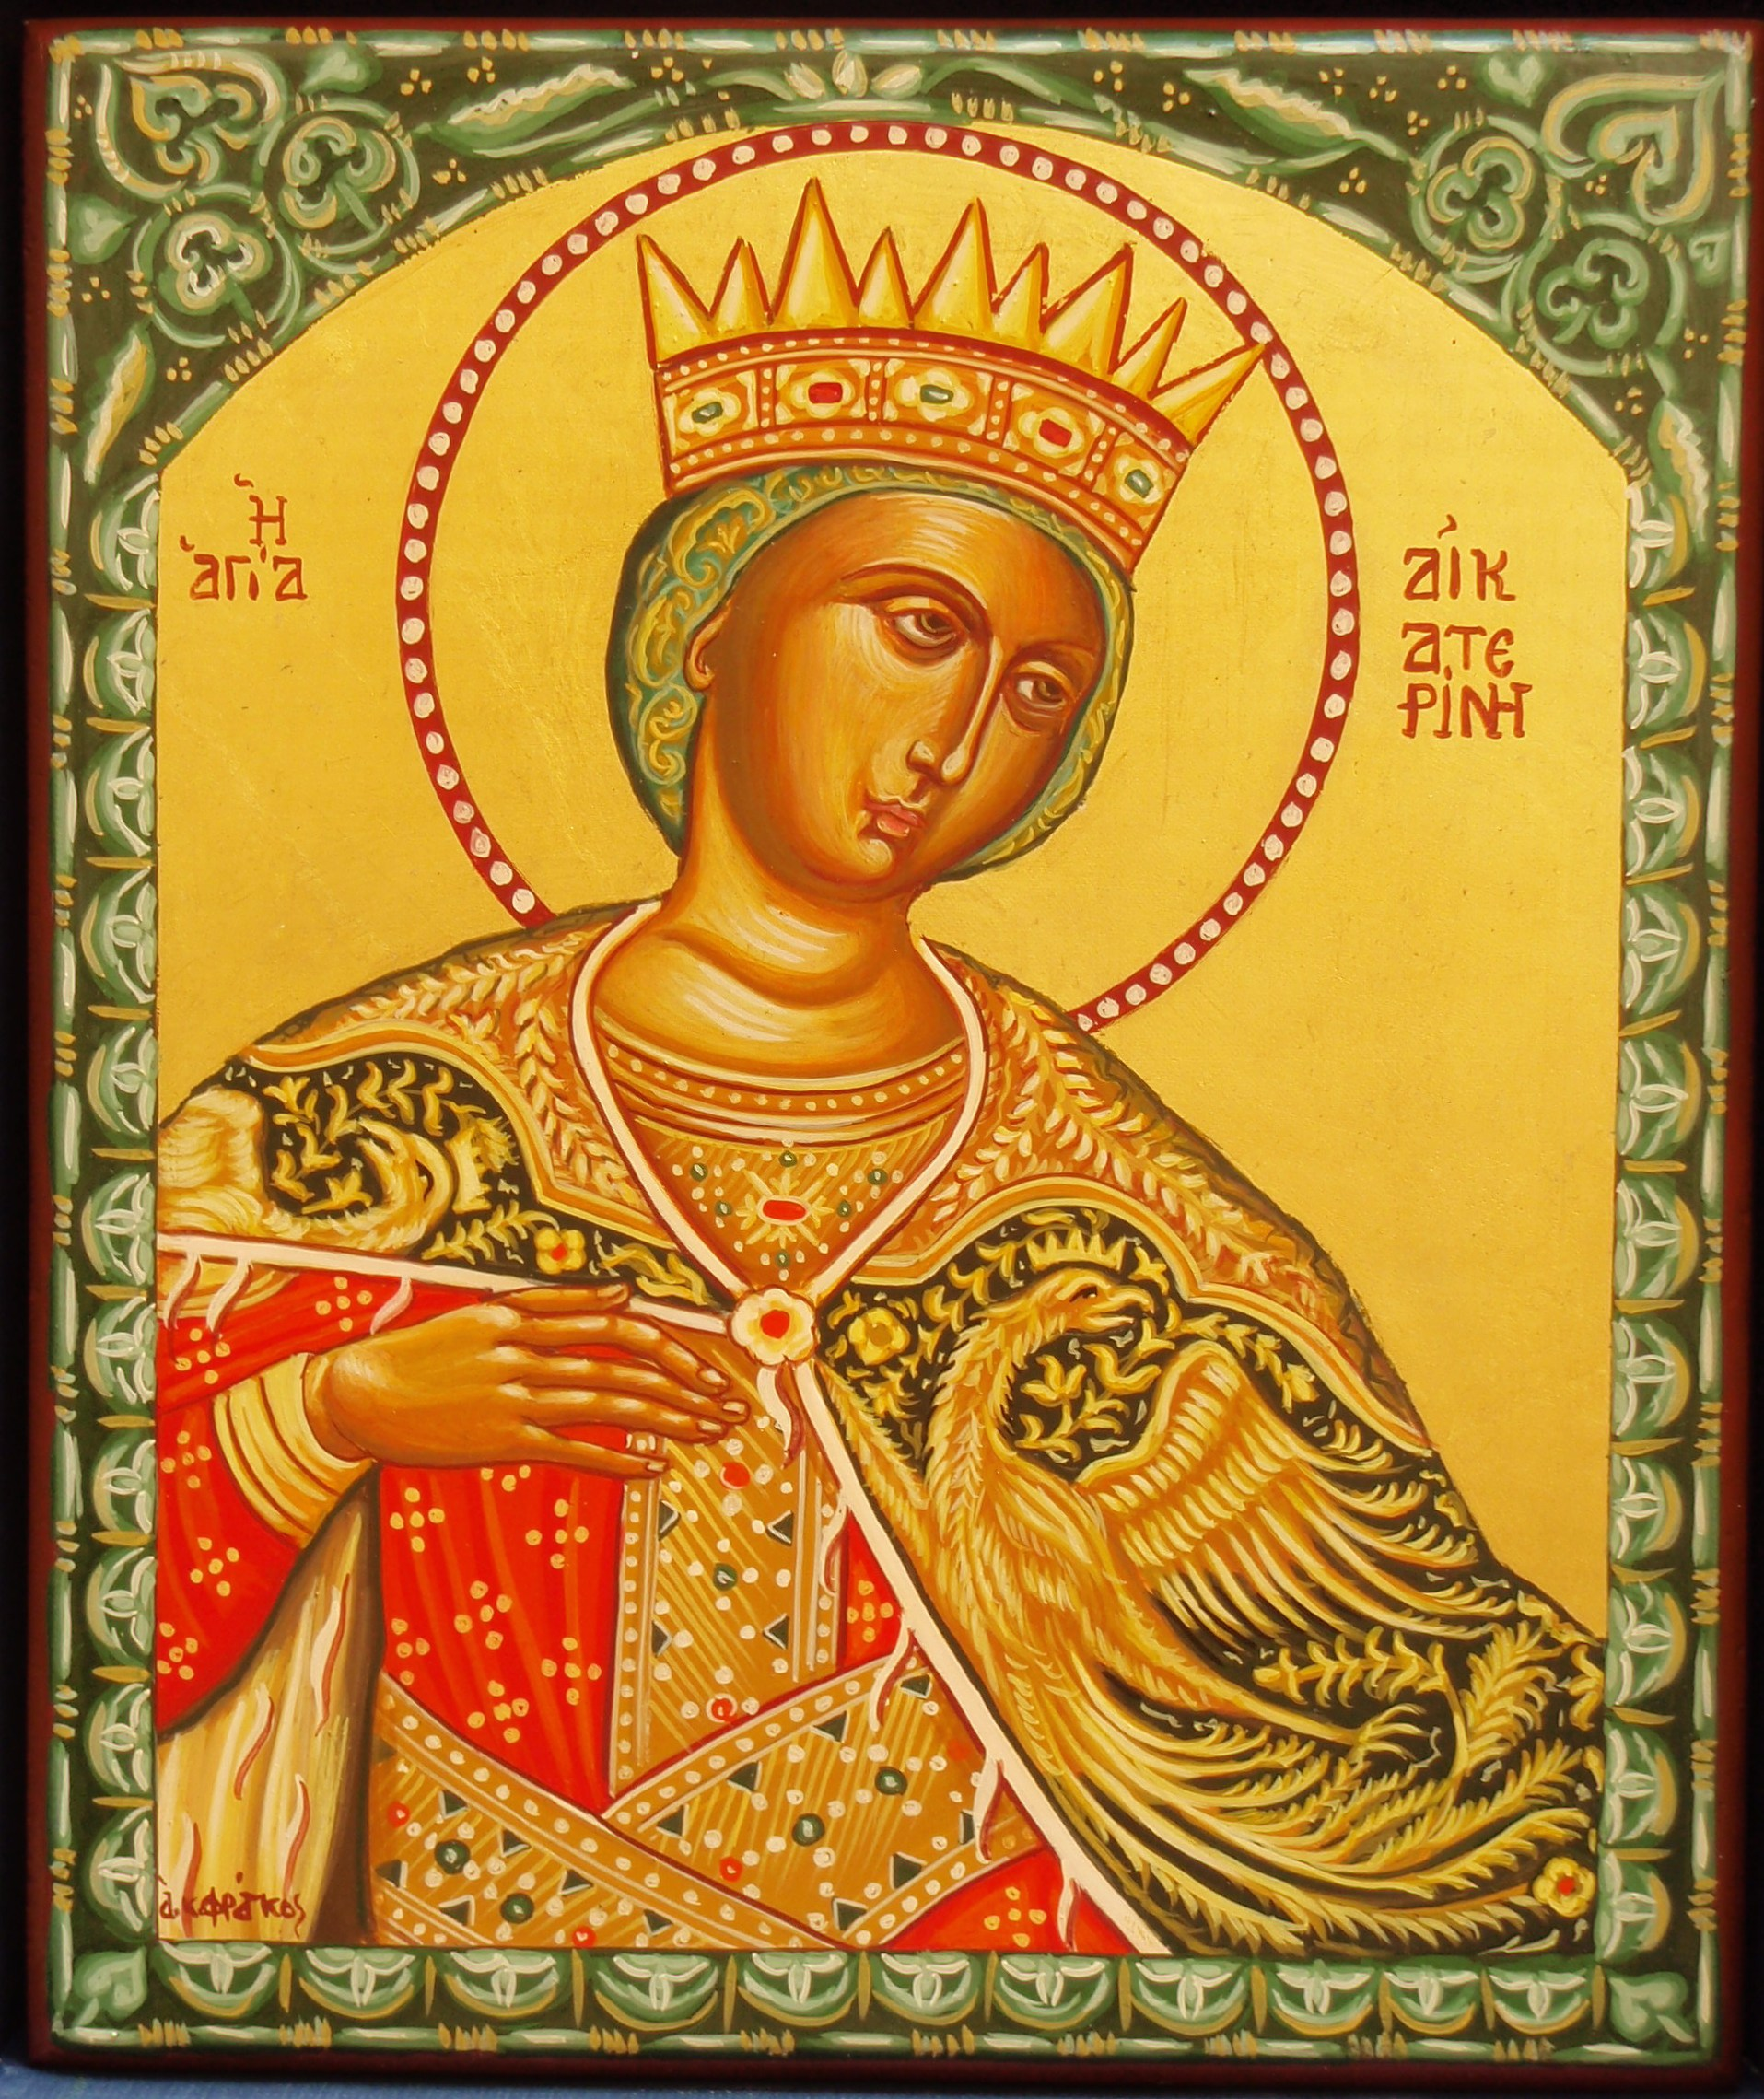
\includegraphics[width=0.5\textwidth]{Katherine1.jpg}}
\date{}
\author{}

\begin{document}
\maketitle
\pagestyle{empty} % Don't show page numbers
\instruction{This page intentionally left blank}
\cleardoublepage
\pagestyle{plain}
\setcounter{page}{1} % Set the page counter to 1 on the first real page
\chapter*{Service of Typica on Palm Sunday \\ Entrance of Our Lord Jesus Christ into Jerusalem}
\readerline{Through the prayers of our holy fathers, Lord Jesus Christ our God,
  have mercy on us, and save us}
\lilypondfile{./Z-Responses/Obikhod/Amen.ly}

\trisagionNeedsAmen[reader]
\lilypondfile{./Z-Responses/Obikhod/Amen.ly}


\centeredsection{The First Antiphon}
\lilypondfile{./Liturgy/B-FirstAntiphon/BlessTheLord_Greek-Music.ly}

\centeredsection{The Second Antiphon}
\lilypondfile{./Liturgy/C-SecondAntiphon/PraiseTheLord_Greek-Music.ly}

\centeredsection{The Third Antiphon}
\lilypondfile{./Liturgy/D-ThirdAntiphon/Beatitudes_Moscow-Music.ly}

\centeredsection{The Epistle}

\instruction{Both of the New Testament lessons are read
without liturgical introduction or conclusion.
The readers start with “The Reading from…” and proceeds}

\paragraph{The Reading from the Epistle of St. Paul to the Philippians. (4:4-9)}\mbox{}\\

Brethren, rejoice in the Lord always; again I will say, Rejoice. Let all men know your
forbearance. The Lord is at hand. Have no anxiety about anything, but in everything by prayer and
supplication with thanksgiving let your requests be made known to God. And the peace of God,
which passes all understanding, will keep your hearts and your minds in Christ Jesus. Finally,
brethren, whatever is true, whatever is honorable, whatever is just, whatever is pure, whatever is
lovely, whatever is gracious, if there is any excellence, if there is anything worthy of praise, think
about these things. What you have learned and received and heard and seen in me, these do; and
the God of peace will be with you.

\centeredsection{The Gospel}

\instruction{Both of the New Testament lessons are read
without liturgical introduction or conclusion.
The readers start with “The Reading from…” and proceeds}

\paragraph{The Reading from the Holy Gospel according to St. John. (12:1-18)}\mbox{}\\

Six days before the Passover, Jesus came to Bethany, where Lazarus who had died was,
whom Jesus had raised from the dead. There they made Him a supper; Martha served, and Lazarus
was one of those at table with Him. Mary took a pound of costly ointment of pure nard and anointed
the feet of Jesus and wiped His feet with her hair; and the house was filled with the fragrance of
the ointment. But Judas Iscariot, Simon’s son, one of His Disciples (he who was to betray Jesus),
said, “Why was this ointment not sold for three hundred denarii and given to the poor?” This he
said, not because he cared for the poor but because he was a thief, and as he had the moneybox he
used to take what was put into it. Jesus said, “Let her alone, let her keep it for the day of My burial.
The poor you always have with you, but you do not always have Me.” When the great crowd of
the Jews learned that He was there, they came, not only on account of Jesus but also to see Lazarus,
whom Jesus had raised from the dead. So the chief priests planned to put Lazarus also to death,
because on account of him many of the Jews were going away and believing in Jesus. The next
day a great crowd who had come to the feast heard that Jesus was coming to Jerusalem. So they
took branches of palm trees and went out to meet him, crying, “Hosanna! Blessed is He Who
cometh in the Name of the Lord, the King of Israel!” And Jesus found a young ass and sat upon it;
as it is written, “Fear not, daughter of Zion; behold, your king is coming, sitting on an ass’s colt!”
His Disciples did not understand this at first; but when Jesus was glorified, then they remembered
that this had been written of Him and had been done to Him. The crowd that had been with Jesus
when He called Lazarus out of the tomb and raised him from the dead bore witness. The reason
why the crowd went to meet Jesus was that they heard He had done this sign.

\centeredsection{Troparia Before the Creed}
\instruction{Plain reading}
\begin{reader}
\item[Reader 1:] The heavenly choir singeth thy praises, saying:
  Holy, holy, holy, Lord of Sabaoth; heaven and earth are full of Thy glory.

\item[Reader 2:] \emph{Come unto him, and be enlightened,
               and your faces shall not be ashamed.}
  The heavenly choir singeth thy praises, saying:
  Holy, holy, holy, Lord of Sabaoth; heaven and earth are full of Thy glory.

\item[Reader 1:] \emph{\glory}
  The choir of the holy angels and archangels,
  with all the powers of heaven, singeth thy praises, saying:
  Holy, holy, holy, Lord of Sabaoth; heaven and earth are full of Thy glory.

\item[Reader 2:]\emph{\nowandever}
\end{reader}

\centeredsection{The Creed}
\input{Common/TheCreed.txt}


\centeredsection{Prayer of Forgiveness}
\readerline{Forgive, remit, pardon, O God, our sins,
  both voluntary and involuntary, in deed and in word, in knowledge or in ignorance,
  committed by night or by day, in mind and in thought.
  Forgive us them all, for thou art good and lovest mankind.
}


\centeredsection{The Lord’s Prayer}
\input{Common/LordsPrayer.txt}

\readerline{Through the prayers of our holy fathers, Lord Jesus Christ our God, have mercy on us.}
\lilypondfile{./Z-Responses/Obikhod/Amen.ly}


\centeredsection{Kontakia for Palm Sunday in Tone Six}
\lilypondfile{./Triodion/PalmSunday/PalmSunday-Kontakion-T6-ByzChant-Music.ly}


\readerline{\lhmForty}

\readerline{
  O Christ our God, Who art worshipped and glorified at all times at every hour both in
  heaven and on earth; Who art long-suffering and plenteous in mercy and compassion; Who lovest
  the just man and showest mercy upon the sinner; and Who callest all men to repentance through 
  the promise of blessings to come; receive, O Lord, at this very hour our supplications, and direct
  our lives in the way of Thy commandments: sanctify our souls, purify our bodies, set our minds
  aright, cleanse our thoughts; deliver us from all affliction, trouble, and distress; compass us about
  with Thy holy angels, that, guided and guarded by them, we may attain unto the unity of the Faith,
  and to the knowledge of Thine unapproachable glory; for Thou art blessed unto ages of ages. Amen.
}

\begin{reader}
  \item \lhmThree{}\\\emph{\gne{}}
  \item \morehonorablethanthetherubim{}
  \item \throughtheprayers{}
\end{reader}

\begin{maybetwocolumns}
\lilypondfile{./Z-Responses/Obikhod/Amen.ly}

\readerline{\blessedbethename{}\thrice{}}

\centeredsection{Psalm 33}
\input{./Psalms/Psalm033-unknowntrans.txt}

\centeredsection{Psalm 144}
\input{./Psalms/Psalm144-unknowntrans.txt}
\end{maybetwocolumns}

\peopleline{\gne}


\centeredsection{A Homily}
\begin{maybetwocolumns}
\instruction{6th Sunday of lent, fourth Sunday of Quarantine
Accepting the Tension Between Our Expectations and God’s Fulfillment:
Homily for Palm Sunday in the Orthodox Church
Fr. Philip LeMasters, pastor, St. Luke Antiochian Orthodox Church of Abilene, Texas}

In religion or anything else, we get used to whatever we get used to. We tend to take for granted
whatever becomes normal, expected, and routine in our lives. Once we learn to see ourselves and
the world in a certain way, it is easy to become blind to even the most obvious truths that challenge
our perspective.

The chief priests and Pharisees certainly missed the point of our Lord’s raising of Lazarus from
the dead after four days in the tomb. They were so afraid of losing their own position and power
that they were unable to recognize Him, as Lazarus’ sister Martha did, as “the Messiah, the Son of
God, who is to come into the world.” The Savior showed that He is “the resurrection and the life”
by resurrecting Lazarus, but all that the religious leaders could see was a threat to themselves.
Though they had the great blessings of the Old Testament law and the worship of the Temple in
Jerusalem, they made themselves blind to a Messiah Who was different from what they had
expected.

We see something similar in the crowd’s reaction to the Savior’s triumphant entry into Jerusalem.
They received Him as the Messiah everyone anticipated, a conquering military hero ready to
liberate Israel from the defilement of Roman occupation. “Hosanna! Blessed is He Who comes
in the Name of the Lord, the King of Israel!” The irony is that Christ arrived not as a fierce warrior,
but peaceably on a humble donkey. When in the following days it became clear that He is the
Prince of Peace Whose Kingdom is not of this world, the same crowds yelled “Crucify Him.” The
Roman governor Pontius Pilate quickly saw that there was no reason to do so, but as a practical
administrator, he could tolerate the death of an innocent man more easily than civil unrest.

Irony abounds in the events leading to the Savior’s Passion. Raising a dead man somehow made
people want to kill Him. Those who praised Him enthusiastically on Sunday called for His death
on Friday. He died as a failed Messiah, rejected by Jewish religious leaders and abandoned by His
disciples. When the women went to His tomb, they did so in order to complete the proper burial
rituals for the deceased. They did not expect to find the stone rolled away and the grave empty;
neither did they anticipate the astonishing message of the angel. The tension between what
anyone thought of Jesus Christ and Who He revealed Himself to be in the final days of His earthly
ministry are truly shocking and beyond normal human comprehension.

Our challenge in the coming week is to enter into the tension between our conventional
expectations and the Lord’s strange victory over death through His Cross and empty tomb, for it
is through that tension that He has brought salvation to the world. If we approach His Passion as
simply part of a story that we take for granted because it is so familiar and we have watered it
down to fit our sensibilities, we will miss the point of this week entirely. Instead, we must learn
to see that we have far too much in common with those who wanted a Messiah to serve their
interests in this world. Those who sought Christ’s death were highly religious, upstanding
members of their society, but they were ultimately idolaters of their own will. We must not shy
away from facing the truth that we are often very much like them. As well, we are not much
different from those who denied and abandoned the Savior when things did not go as they had
hoped. There is much within us that wants to run away from the dark night of the Cross and the
grave.

Even though it goes very much against our inclinations, we must struggle to abide with Christ as
He offers up Himself for our salvation to the point of death. We must resist the temptation simply
to disregard Him because we do not like what His Passion reveals about our need for healing that
we cannot give ourselves. We must behold Him in the tomb, facing the astonishing mystery of
the death of the God-Man, of the Eternal Word of God Who spoke the universe into existence, if
we are to share in His great victory over Hades and death itself. We must dare to disorient
ourselves from our usual schedules and preoccupations, turning away from the temptation to make
the world our god and to use religion for our own self-centered purposes.

As we follow our Lord to His Passion this week, we will come face to face with the profound
tension between our ways and God’s ways. We will not merely have thoughts and feelings about
what happened long ago, but will instead enter mystically into Jesus Christ’s great Self-Offering
for our salvation. We will encounter personally the Lamb of God Who takes away the sin of the
world in a way that calls us into question from the depths of our souls. The more fully we open
ourselves to the unfathomable mystery of the God-Man Who enters into death, the more we will
die to the prideful illusions that so easily blind us to the truth about who we are and Who He is.
We will see that conventional religion that helps us get what we want on our own terms in this
world is powerless to deliver us from the clutches of death. Such distorted religion is precisely
why the chief priests and Pharisees rejected their Messiah and insisted on His crucifixion. It is
precisely why they chose death over life. That is a tragic irony that we must avoid, if we are to
share in the eternal life of our Savior, Who triumphs over the worst that corrupt human powers
and death itself can do.

Throughout the coming week, we will have the opportunity to open the eyes of our souls to the
brilliant light of the glory of God, shining from the empty tomb. But in order to do so, we must
first endure the pitch black midnight of the God-Man hanging on the Cross purely out of love for
you, for me, and for everyone He created in His image and likeness. Let us do so in obedience to
the instructions of St. Paul in today’s epistle reading: “Whatever is true, whatever is honorable,
whatever is just, whatever is pure, whatever is lovely, whatever is gracious, if there is any
excellence, if there is anything worthy of praise, think about these things.” Regardless of what
else is going on in our lives in the coming week, there could be nothing more important than
opening our hearts to the Savior Who offered up Himself for our salvation. He alone is able to
bring us all from the dark pit of despair into the blinding light of His Kingdom. Now is the time
to “lay aside all earthly cares” and to attend to Him. “Hosanna! Blessed is He Who comes in the
Name of the Lord, the King of Israel!”

\end{maybetwocolumns}

\centeredsection{Apolytikion of Lazarus Saturday in Tone 1}
\lilypondfile{./Triodion/LazarusSaturday/LazarusSaturday-ByzChant-T1-Music.ly}

\centeredsection{Apolytikion of Palm Sunday in Tone Four}
\lilypondfile{./Triodion/PalmSunday/PalmSunday-Apolytikion-T4-ByzChant-Music.ly}

\vspace{1cm}
\instruction{If your family chooses to process around the exterior of your house,
you can sing the Apolytikia of Lazarus Saturday and Palm Sunday,
“Rejoice, O Bethany” and the Trisagion Hymn}

\readerline{\throughtheprayers}

\lilypondfile{./Z-Responses/Obikhod/Amen.ly}

\end{document}

